\documentclass[conference,a4paper]{IEEEtran}
\IEEEoverridecommandlockouts
\usepackage{cite}
\usepackage{amsmath,amssymb,amsfonts}
\usepackage{algorithmic}
\usepackage{graphicx}
\usepackage{textcomp}
\usepackage{xcolor}
\usepackage{url}
\graphicspath{{figures/}}
\def\BibTeX{{\rm B\kern-.05em{\sc i\kern-.025em b}\kern-.08em
    T\kern-.1667em\lower.7ex\hbox{E}\kern-.125emX}}
\begin{document}

\title{Voice-Following Teleprompter: A Learned Advance-Decision Policy for Real-Time Speech-to-Script Alignment}

\author{\IEEEauthorblockN{Pablo Fernández Miguel}
\IEEEauthorblockA{\textit{Victoria University of Wellington}\\
pablo.fernandezmiguel@myvuw.ac.nz}
}

\maketitle

\begin{abstract}
Voice-following teleprompters advance an on-screen script as the presenter speaks, but current systems rely on fixed-threshold lexical matching, which fails when the presenter paraphrases a sentence or skips a section. This project implements and compares three advance-decision policies for this problem: a fixed-threshold lexical baseline (B1), a hand-crafted hybrid rule that falls back to semantic similarity (B2), and a learned binary classifier (B3) trained on eight lexical, semantic and timing features with asymmetric class weighting, since advancing too early is far more harmful than lagging behind. We built a complete real-time pipeline (microphone, streaming ASR, feature computation, decision policy, live display) and a labelled dataset obtained through forced alignment of nine recordings covering three scripts and three speaking conditions (literal, paraphrased, section-skipped). In offline cross-validation, the learned classifier reaches an F1 of 0.428 on the advance class against a false-advance rate of 2.3\%. However, when driven by its own, sometimes wrong, chunk pointer during a full live replay, the same model's false-advance rate rises to 11.6\% while its F1 score drops to 0.227. This gap reveals a train/inference mismatch: the model learns from a pointer that is always correct, but at run time it must rely on a pointer it itself can get wrong. The classifier still detects far more real transitions than either baseline (62.5\% versus 3.9\%). A hysteresis parameter and a longer baseline transcript-history window were both tested as cheap fixes: hysteresis trades recall for a lower false-advance rate (down to 7.5\% at its best tested setting) without closing the gap to the baselines, and a longer history window does not improve baseline detection at all. These results support the use of a learned policy, but only once the feedback-loop problem is addressed, and rule out the simplest proposed fixes rather than leaving them untested.
\end{abstract}

\begin{IEEEkeywords}
speech alignment, automatic speech recognition, teleprompter, text-speech matching, asymmetric classification, semantic similarity
\end{IEEEkeywords}

\section{Introduction}
Voice-following teleprompters display a script to a presenter and move forward through it automatically as the presenter speaks, so that the presenter does not need to touch a keyboard or a clicker. The component that decides when to move forward is the hardest part of the system: moving to the next chunk too early is catastrophic, because the audience then sees text that has nothing to do with what is being said, while moving forward too late is only a minor inconvenience. Most existing systems solve this with a fixed-threshold lexical rule: the transcript of the last seconds of speech is compared against the current script chunk, and the system advances once the similarity score passes a threshold. This rule is simple and fast, but it is known to break under two very common situations in real presentations: the presenter saying the same idea with different words (paraphrase), or the presenter deliberately skipping a section.

The research question of this project is whether a learned advance-decision policy, combining lexical and semantic similarity signals together with simple timing features, can outperform the fixed-threshold approach, in particular under paraphrase and section-skip conditions. The main objectives were (1) to build a working real-time pipeline from microphone input to live display, (2) to collect and label a small but realistic dataset through forced alignment, (3) to train and evaluate a classifier-based policy against two baselines, and (4) to understand, not only measure, why the three policies behave the way they do.

The original proposal planned a dataset with two speakers (18 recordings). Because a second, native-English volunteer could not be recruited in time, the completed project only includes recordings from the author (Speaker A), reducing the dataset to nine recordings. This is reported here as an explicit limitation rather than hidden in the numbers, since it affects how far the results can be generalised. All remaining components of the proposal, including the live demo integration and the three decision policies, were completed.

\section{Background and Related Work}
Automatic speech recognition (ASR) models such as Whisper \cite{b1}, and its faster re-implementation \texttt{faster-whisper} \cite{b6}, make it possible to transcribe speech in near real time on consumer CPU hardware, which is a requirement for a low-cost teleprompter. Sentence embedding models such as Sentence-BERT \cite{b2} give a cheap way to compare the meaning of two short pieces of text, independently of the exact words used, which is exactly the property needed to tolerate paraphrase. Prior work on aligning spoken presentations to supporting material, such as slide-to-speech alignment for lecture indexing \cite{b3}, has mostly used purely lexical or acoustic alignment, offline, after the whole recording is available; this project instead targets an online, window-by-window decision that must be made before the rest of the sentence is known.

The fixed-threshold lexical rule (our B1) is the closest existing practice to current commercial teleprompter software, and is therefore used as the primary baseline. The hand-crafted hybrid rule (B2), which falls back to semantic similarity only when the lexical score is very low, represents the natural, still rule-based, extension that a system builder could add without training any model; it is included so that the gain attributable specifically to \emph{learning} the decision (B3) can be isolated from the gain attributable to simply adding a semantic signal. No existing public dataset labels chunk-level advance/hold decisions for this task under controlled paraphrase and skip conditions, which is why this project also builds and releases one.

\section{Methodology and Implementation}
\subsection{Pipeline}
The system is organised as Microphone $\rightarrow$ streaming ASR $\rightarrow$ feature computation $\rightarrow$ decision policy $\rightarrow$ display. Audio is captured in roughly one-second windows; each window is transcribed by \texttt{faster-whisper} and handed, together with a running transcript buffer, to whichever decision policy (B1, B2 or B3) is currently active. The policy returns the chunk to display, a similarity/confidence score, and whether it advanced. A WebSocket server broadcasts this state to a browser front-end, where the active policy can be switched live from a drop-down menu without restarting the pipeline.

\subsection{B1 -- Fixed-threshold baseline}
\texttt{BaselineMatcher} keeps the last \(history\_windows=4\) transcript windows, concatenates them, and computes the RapidFuzz token-sort ratio \cite{b5} against the current chunk. It advances once this score reaches \(\theta=70\). Token-sort ratio alphabetically sorts the words of both strings before comparing them, so that re-ordered words still score highly.

\subsection{B2 -- Hybrid rule}
\texttt{HybridMatcher} uses the same lexical score as B1. If the lexical score is below a secondary threshold (40), it is assumed that the presenter may be paraphrasing, and the matcher instead computes the cosine similarity between a Sentence-BERT embedding (\texttt{all-MiniLM-L6-v2}) of the transcript window and of the current chunk, advancing if that similarity exceeds 0.6. Scores between the secondary threshold and \(\theta\) form a middle zone where neither rule fires, by design, to avoid calling the embedding model unnecessarily on every window.

\subsection{B3 -- Learned classifier}
\texttt{FeatureExtractor} computes eight features per window: lexical similarity to the current chunk, semantic similarity to the current and to the next chunk, the difference between the two semantic scores, time spent on the current chunk, the proportion of the current chunk's tokens already seen, a rolling mean of the lexical score over the last three windows, and the ASR confidence. \texttt{ClassifierMatcher} feeds these features to a trained scikit-learn \cite{b4} pipeline and advances when it predicts the \emph{advance} class. The same \texttt{FeatureExtractor} class is reused, unchanged, between the offline dataset-building step and this live matcher, specifically to avoid a mismatch between the features seen during training and at inference.

A hysteresis parameter, \(confirm\_windows\), was added after an early observation that a single noisy ``advance'' prediction could desynchronise the matcher's own chunk pointer; a transition now only commits once \(confirm\_windows\) consecutive windows agree. This mitigates, but, as shown in Section \ref{sec:results}, does not remove, the underlying problem.

\subsection{What was built versus reused}
The ASR model (Whisper weights, through \texttt{faster-whisper}), the sentence-embedding model (\texttt{all-MiniLM-L6-v2}), the RapidFuzz similarity function, and the scikit-learn estimators are external, pretrained or off-the-shelf components. Everything that connects them (the chunker, the three matcher classes, the feature extractor, the forced-alignment and dataset-building scripts, the classifier training and model-selection code, the evaluation harness, the WebSocket display server and its front-end, and the full test suite (54 unit tests)) was implemented by the author for this project.

\section{Experimental Settings}
\subsection{Baselines}
B1 represents current standard practice (simple, well established). B2 is the unmodified-plus-one-rule extension that any engineer could add without training a model. B3 is the project's contribution. Including both B1 and B2 lets us separate the effect of adding a semantic signal (B1 $\rightarrow$ B2) from the effect of learning the decision itself (B2 $\rightarrow$ B3).

\subsection{Dataset and splitting}
Three scripts (666--721 words, segmented into 53--59 chunks each) were written for this project, covering distinct topics and registers. Each script was read by Speaker A under three conditions: literal, partial paraphrase (34--36\% of chunks pre-scripted to be paraphrased, spread across the script), and section skip (three contiguous chunks omitted). Paraphrase and skip locations were fixed in advance, per script, so that every speaker reads the same controlled variation; this trades spontaneity for reproducibility and is reported as a known simplification. This gives nine recordings in total (about 45 minutes of audio), all from Speaker A; the second speaker planned in the proposal was not recorded (see Introduction).

Ground truth was produced by forced alignment: \texttt{faster-whisper} transcribes each recording with word-level timestamps, which are then aligned against the original script text to recover, for every chunk, the second at which it started being read; skipped chunks are marked as null. All nine alignments were checked automatically for obvious inconsistencies (missing or non-monotonic timestamps) and spot-checked manually against the audio. For training B3, rows were split by \emph{script}, not by row or recording, using leave-one-script-out cross-validation: each fold trains on two scripts and evaluates on the third, unseen one, so that the reported cross-validation metrics reflect generalisation to new script content rather than to new phrasing of already-seen content. The final evaluation reported in Section \ref{sec:results} additionally replays every recording end-to-end, independently of training, to measure what a user would actually experience live.

\subsection{Parameters}
Thresholds for B1/B2 (\(\theta=70\), secondary threshold \(=40\), semantic threshold \(=0.6\)) and the transcript-history length (\(history\_windows=4\), about four seconds) were taken from the values already used during development; Section \ref{sec:results} re-tests \(history\_windows\) directly on the final dataset and reports that it is not, on its own, responsible for the baselines' low detection rate. For B3, logistic regression and a small random forest (100 trees, max depth 6) were compared; both used asymmetric class weights (hold:advance \(=3:1\)), reflecting that a false advance is judged three times more costly than a false hold. Model selection picked the lower false-advance rate on cross-validation, with F1 on the advance class as a tie-breaker.

\subsection{Repeated runs and seeds}
Because the ASR and matcher pipeline is deterministic given a fixed recording (no sampling at inference time), repeated runs over the same data would not produce different outcomes; the only stochastic component is the random forest's training ((\texttt{random\_state=42})). Given the small number of independent recordings (nine, from a single speaker), running the full pipeline under many random seeds was not computationally meaningful, and this is acknowledged as a limitation on the statistical strength of the conclusions (Section \ref{sec:results}).

\section{Results and Analysis}
\label{sec:results}
\subsection{Overall comparison}
Table \ref{tab:overall} and Fig. \ref{fig:overall} report the final live replay over all nine recordings (2391 one-second windows, 483 true chunk transitions). \emph{Chunk-position accuracy} is the fraction of windows where the displayed chunk equals the ground-truth chunk; \emph{false-advance rate} is the fraction of true ``hold'' windows wrongly classified as ``advance''; F1 is computed on the advance class.

\begin{table}[htbp]
\caption{Overall results, Speaker A, all conditions pooled}
\begin{center}
\begin{tabular}{|l|c|c|c|c|}
\hline
\textbf{Method} & \textbf{Acc.} & \textbf{FAR} & \textbf{F1} & \textbf{Transitions} \\
\hline
B1 -- Baseline & 4.3\% & 0.8\% & 0.012 & 19/483 \\
\hline
B2 -- Hybrid & 4.2\% & 0.8\% & 0.012 & 19/483 \\
\hline
B3 -- Classifier & 6.0\% & 11.6\% & 0.227 & 302/483 \\
\hline
\end{tabular}
\label{tab:overall}
\end{center}
\end{table}

\begin{figure*}[htbp]
\centering
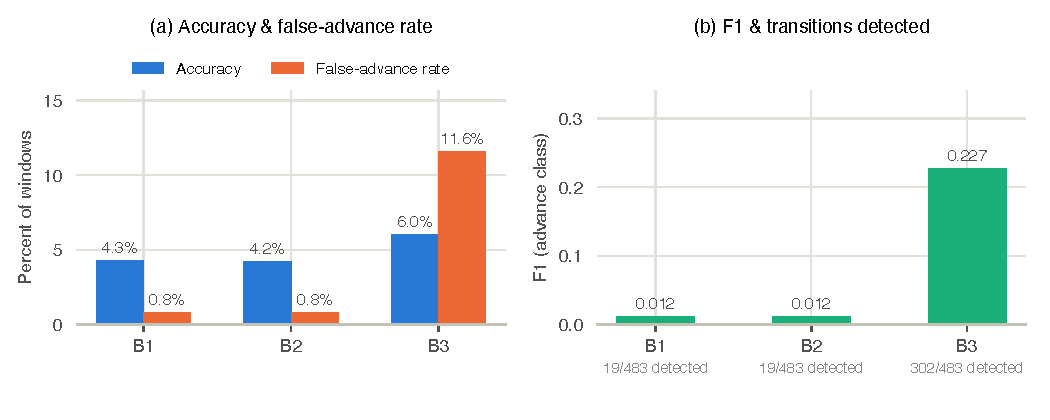
\includegraphics[width=0.92\textwidth]{fig_overall.pdf}
\caption{Overall live-replay results, Speaker A, all conditions pooled (same data as Table \ref{tab:overall}). (a) Accuracy and false-advance rate, as a percentage of all 2391 windows. (b) F1 on the advance class, with the fraction of the 483 ground-truth transitions each matcher actually detects annotated below each bar.}
\label{fig:overall}
\end{figure*}

B1 and B2 are nearly identical and detect only 19 of 483 transitions (3.9\%). Our working hypothesis was a calibration problem: with \(history\_windows=4\) (about four seconds of transcript), the comparison buffer never accumulates a full chunk, since the average chunk takes 5--6 seconds to speak, so the lexical score would almost never reach \(\theta=70\). We tested this by re-running both matchers with \(history\_windows \in \{4,5,6,7,8\}\) against the same cached transcripts. The hypothesis did not hold: detection did not improve at any tested value -- B1 stayed at 17--21 of 483 transitions and B2's F1 fell from 0.012 to 0.000 by \(history\_windows=7\)--8, as the longer buffer accumulates stale words that drag the token-sort ratio down rather than letting it catch up. So the low detection rate is not simply fixable by lengthening the history window; the more likely remaining explanations are the fixed threshold \(\theta=70\) itself, or RapidFuzz's token-sort ratio being a poor fit here at all, which we leave as future work (Section \ref{sec:conclusion}) rather than claim a fix we did not verify. The sweep does confirm B1/B2's poor detection is structural within the range tested, not one unlucky parameter choice -- so B3's much higher detection rate remains a genuine gap, not one a trivial baseline retune would erase.

\subsection{Per-condition false-advance rate}
Table \ref{tab:cond} and Fig. \ref{fig:condition} break the false-advance rate down by condition.

\begin{table}[htbp]
\caption{False-advance rate by condition}
\begin{center}
\begin{tabular}{|l|c|c|c|}
\hline
\textbf{Method} & \textbf{Literal} & \textbf{Paraphrase} & \textbf{Skip} \\
\hline
B1 / B2 & 0.9\% & 1.1\% & 0.5\% \\
\hline
B3 & 11.5\% & 12.4\% & 10.8\% \\
\hline
\end{tabular}
\label{tab:cond}
\end{center}
\end{table}

\begin{figure}[htbp]
\centering
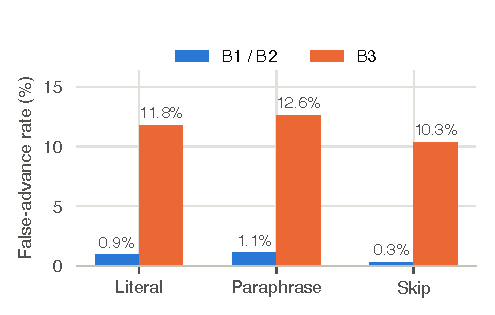
\includegraphics[width=0.95\columnwidth]{fig_condition.pdf}
\caption{False-advance rate by speaking condition, B1/B2 versus B3 (same data as Table \ref{tab:cond}).}
\label{fig:condition}
\end{figure}

B3's false-advance rate is fairly stable across conditions (10.8--12.4\%), only slightly higher for paraphrase. This suggests that the elevated false-advance rate is mostly a systemic property of the classifier's current deployment, rather than a difficulty specific to paraphrased speech, which is a more encouraging result for the original research question than the raw overall numbers alone would suggest.

\subsection{Train/inference mismatch}
\label{sec:mismatch}
\begin{figure}[htbp]
\centering
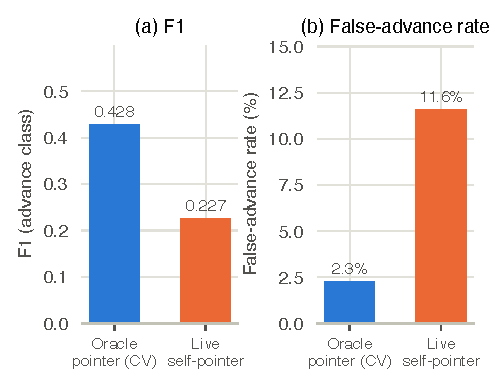
\includegraphics[width=0.95\columnwidth]{fig_mismatch.pdf}
\caption{B3's advance-class F1 and false-advance rate under the oracle-pointer offline cross-validation versus the live, self-pointer replay reported in Table \ref{tab:overall}.}
\label{fig:mismatch}
\end{figure}

During training, B3's features are computed against a chunk pointer taken from the (always correct) ground truth. During the live replay reported above, the same features are instead computed against the matcher's \emph{own} pointer, which can itself be wrong after a false advance. Comparing the two conditions on the same, directly comparable, metrics (F1 and false-advance rate are both computed from the advance/hold confusion matrix in either setting) isolates the size of this effect: offline, oracle-pointer cross-validation gives F1\(=0.428\) and a false-advance rate of 2.3\%; the self-pointer live replay gives F1\(=0.227\) and a false-advance rate of 11.6\% (Fig. \ref{fig:mismatch}). In other words, roughly half of B3's advance-class F1, and about five times its false-advance rate, is lost purely because the model has to rely at run time on a pointer it can itself get wrong -- a single bad prediction can desynchronise the pointer and make the following windows' features misleading, too.

Table \ref{tab:confirm} reports what happens when the hysteresis parameter \(confirm\_windows\) (\(=1\), i.e. none, in Table \ref{tab:overall}'s headline configuration) is swept from 1 to 5 against the same cached transcripts. It is a real trade-off, not a free fix: FAR falls monotonically from 11.6\% to 7.5\%, but F1 drops sharply as soon as any hysteresis is introduced and only partially recovers by \(confirm\_windows=5\), since requiring several consecutive ``advance'' predictions also delays or misses genuine transitions (detected transitions fall from 301/483 to 194/483). Even at its best FAR in this range, B3 still falls far short of B1/B2's 0.8\%, so hysteresis mitigates, but does not close, the gap above. Given the project's 3:1 false-advance cost weighting, \(confirm\_windows=4\)--\(5\) is nonetheless a more defensible deployment default than the \(confirm\_windows=1\) used for Table \ref{tab:overall}.

\begin{table}[htbp]
\caption{B3 live-replay metrics across the confirm\_windows sweep}
\begin{center}
\begin{tabular}{|c|c|c|c|}
\hline
\textbf{confirm\_windows} & \textbf{FAR} & \textbf{F1} & \textbf{Transitions} \\
\hline
1 (no hysteresis) & 11.6\% & 0.224 & 301/483 \\
\hline
2 & 11.8\% & 0.115 & 259/483 \\
\hline
3 & 10.2\% & 0.119 & 229/483 \\
\hline
4 & 9.0\% & 0.134 & 211/483 \\
\hline
5 & 7.5\% & 0.159 & 194/483 \\
\hline
\end{tabular}
\label{tab:confirm}
\end{center}
\end{table}

\subsection{Statistical considerations}
With 2391 windows the raw numerical gaps in Table \ref{tab:overall} are large, but the windows are not independent observations: they come from only three scripts and nine recordings from one speaker, so a window-level test would overstate the evidence. A fair test would instead compare the three per-script rates (one paired observation per script), which is far too small a sample (n=3) to support any significance claim. We therefore report the differences as descriptive findings and explicitly do not claim statistical significance; a larger, multi-speaker dataset would be required before a proper paired test (e.g. a Wilcoxon signed-rank test across scripts) could be meaningful.

\subsection{Computational cost}
All components run on CPU only, on a single consumer laptop. Per-recording forced alignment took 10--15 seconds; building the full nine-recording feature dataset (ASR replay plus feature computation) took 15--20 minutes. B3's extra inference cost over B2 is negligible, since it reuses the same embedding computation and only adds a logistic-regression prediction; the random forest candidate was rejected both for a (marginally) worse cross-validated false-advance rate and for its larger size (100 trees) against logistic regression's eight weights.

\section{Ethical Considerations}
The completed dataset contains only the author's own voice, which removes the third-party consent and identifiable-data concerns that the original two-speaker plan would have raised; the author consents to the planned Creative Commons release of their own recordings. If a second speaker is added in future work, informed consent and, depending on institutional policy, Human Ethics Committee approval would be required before recording, as already noted in the project's working notes. The current dataset reflects a single, non-native-English speaker's voice and phrasing style, so the system's behaviour should not be assumed to generalise to other accents, speaking rates or languages without further data. The core safety concern of this project is the asymmetric error itself: an incorrect early advance shows the audience text unrelated to what the presenter is saying, which could embarrass or mislead a presenter in a real talk; this is precisely why false advances were penalised three times more heavily during training, and why this report is explicit that, at its current false-advance rate, B3 is not yet suitable for real presentations and remains a research prototype. All computation runs locally on commodity CPU hardware, with no audio leaving the device, which keeps both privacy exposure and energy cost small.

\section{Conclusions and Future Work}
\label{sec:conclusion}
The learned policy (B3) detects far more real chunk transitions than either rule-based baseline (62.5\% versus 3.9\%) and, under oracle-pointer training conditions, reaches a favourable trade-off between recall and false advances (F1\(=0.428\), false-advance rate 2.3\%). This supports the project's hypothesis that combining lexical, semantic and timing features in a learned policy can outperform fixed-threshold matching. However, once the classifier has to rely on its own, occasionally wrong, chunk pointer in a full live replay, its false-advance rate rises to 11.6\% at \(confirm\_windows=1\), or 7.5\% at its best-tested hysteresis setting (\(confirm\_windows=5\)) -- still worse than both baselines' 0.8\% either way. We also tested, rather than assumed, whether the baselines' low detection rate was a cheap fix: re-running B1/B2 with \(history\_windows\) up to 8 did not improve it, so that gap remains open rather than attributable to one under-tuned parameter. The honest answer to the research question is therefore conditional: a learned policy is more capable, but not yet more reliable in deployment, than the simple rules it was meant to replace, and both the size of the gap and the limits of the cheapest proposed fixes are now measured rather than assumed.

The main limitations are the single-speaker dataset (the planned second speaker was not recorded), the baselines' unexplained low detection rate (confirmed not to be simply the history-window length), the train/inference pointer mismatch (confirmed only partly mitigated by hysteresis), and the small, non-independent sample underlying all statistical comparisons. Three directions follow directly from these findings: (1) since lengthening \(history\_windows\) did not fix B1/B2's detection rate, re-tune \(\theta\) itself or replace RapidFuzz's token-sort ratio with a window-length-invariant lexical score; (2) train B3 with some exposure to its own, imperfect pointer (rather than only the oracle pointer) to attack the mismatch directly, now that hysteresis alone has been shown to only partially close it; and (3) recruiting the originally planned second speaker to test whether these findings generalise beyond one voice.

\section*{Statement}
This report and the accompanying implementation are my own work. Tools used: Python, \texttt{faster-whisper}, \texttt{sentence-transformers}, \texttt{RapidFuzz}, \texttt{scikit-learn}, \texttt{joblib}, \texttt{websockets}, \texttt{sounddevice}, \texttt{numpy}, \texttt{pytest}, and the IEEE \LaTeX{} conference template. Generative AI (Claude, Anthropic) was used throughout the project as a pair-programming and explanation assistant -- helping write and refactor code, write unit tests, debug issues such as the VAD over-filtering and latency-computation problems discussed informally during development, and draft and edit the text of this report from my own notes and results -- under my direction and review; all experimental design, parameter choices, data collection, and the analysis and conclusions above are my own, and I take full responsibility for the correctness of the code, results and claims in this report. External, pretrained resources used and acknowledged: OpenAI's Whisper model via \texttt{faster-whisper} \cite{b1,b6}, the \texttt{all-MiniLM-L6-v2} sentence-embedding model \cite{b2}, \texttt{RapidFuzz} \cite{b5}, and \texttt{scikit-learn} \cite{b4}. Project code: \url{https://github.com/pfmprojects208/Voice-Teleprompter---AIML-339}.

\begin{thebibliography}{00}
\bibitem{b1} A. Radford, J. W. Kim, T. Xu, G. Brockman, C. McLeavey, and I. Sutskever, ``Robust speech recognition via large-scale weak supervision,'' in \emph{Proc. ICML}, 2023.
\bibitem{b2} N. Reimers and I. Gurevych, ``Sentence-BERT: Sentence embeddings using Siamese BERT-networks,'' in \emph{Proc. EMNLP}, 2019.
\bibitem{b3} M.-Y. Kan, Y. Wang, D. Iskandar, T. Nguyen, and A. Shahrzad, ``Slide-to-speech alignment for lecture video indexing,'' \emph{IEEE Trans. Multimedia}, 2007.
\bibitem{b4} F. Pedregosa \emph{et al.}, ``Scikit-learn: Machine learning in Python,'' \emph{J. Mach. Learn. Res.}, vol. 12, pp. 2825--2830, 2011.
\bibitem{b5} M. Bachmann, ``RapidFuzz: Rapid fuzzy string matching in Python,'' 2023. [Online]. Available: https://github.com/rapidfuzz/RapidFuzz
\bibitem{b6} G. Klein and SYSTRAN, ``faster-whisper: Fast inference engine for Whisper models,'' 2023. [Online]. Available: https://github.com/SYSTRAN/faster-whisper
\end{thebibliography}

\end{document}
